\chapter[Introduction to the Template: Motivation and First Steps]{Introduction to the Template Motivation and Steps}
\label{cp:introduction}

{
  \parindent0pt

  \textit{Author: Gaurav Raj}

  \textit{License: \LaTeX~GPLv3}

  \textit{Official Repository: \href{https://github.com/thehackersbrain/thesis-template}{GitHub Repository}}

  \vspace{.935em}

  Welcome to the \textcolor{maincolor}{\textit{Thesis Template}} template! Thank you for choosing it for your dissertation, report, or project. This template reflects many hours of development, and I hope you enjoy using it as much as I did creating it. This chapter introduces its purpose and helps you get started. See \autoref{cp:user-guide} for a detailed guide, and \autoref{cp:latex-tutorial} for a brief \LaTeX~tutorial to maximise its use.
}

\section{Motivation}
Modern operating systems abstract hardware complexity through layers of device drivers, system calls, and memory management frameworks. While this abstraction enables application portability and developer productivity, it obsecures the fundamental hardware-software interface that defines computing. Understanding this interface -- how instructions execute, how memory is addressed, how peripherals communicate with the CPU--remains essential for systems programmers, security researchers, and anyone seeking to master computer architecture at its lowest level.

Building an operating system from scratch forces direct engagement with these fundamentals. There are no libraries to mask segmentation faults, no kernel panic handlers to catch undefined behavior, and no scheduler to hide the cost of context switches. Every function call maps to assembly instructions, every pointer dereference translates to physical memory access, and every hardware interaction requires manual register manipulation.

\textbf{THBOS} (\textit{TheHackersBrain Operating System}) was conceived as a minimal x86 kernel that prioritizes transparency over functionality. Rather than implementing a full-featured environment, THBOS focuses on direct CPU interaction through the CPUID instruction, providing real-time hardware introspection while maintaining a codebase small enough to audit in a single sitting. The entire kernel—boot loader, VGA driver, and CPUID wrapper—comprises fewer than 500 lines of combined C and Assembly.

This is a complete expermentation project while learning and keeping things practical for everyone.

\section{Another Important Note}
Okay, My emacs setup is finally working and is awesome.

\newpage

\section{Maths Testing}
This is the section to plot maths graphs.

\vspace{10pt}

\begin{figure}[h]
  \begin{center}
    \begin{tikzpicture}
      \begin{axis}[
          axis lines=middle,
          xlabel={$t$},
          ylabel={$v$},
          xmin=-0.2, xmax=1,
          ymin=-40, ymax=70,
          xtick={0},
          ytick={-30,0,60},
          width=10cm,
          height=8cm,
          axis line style={->},
          ticklabel style={font=\small}
        ]

        \addplot[domain=0:0.5, thick]{60};
        \addplot[domain=0:0.5, thick, dashed]{-30};

        \draw[dashed] (axis cs:0.5,0) -- (axis cs:0.5,-30);
        \draw[dashed] (axis cs:0.5,60) -- (axis cs:0.5,0);

        \node at (axis cs:0.5,62) [anchor=west] {$v = \SI{60}{\metre\per\second}$};
        \node at (axis cs:0.5,-30) [anchor=west] {$v = -30$};
        \node at (axis cs:0.25,30) {Area 30};
        \node at (axis cs:0.25,-15) {Area -15};
        \node at (axis cs:0.5,0) [below, xshift=6pt] {$\tfrac{1}{2}$};

      \end{axis}
    \end{tikzpicture}
  \end{center}
\end{figure}
\vspace{10pt}

\subsection{Function Plots}

You think trigonometry is only for navigaters. Think again. Some of the best use cases of trigonometry is in \textbf{\textit{rotation}}, \textbf{\textit{vibration}}, and \textbf{\textit{Oscillation}}. Basically in repeating patterns or motions.

\vspace{\baselineskip}

Here's a simple \textbf{\textit{Sinusoidal Oscillation}}.

\vspace{10pt}

\begin{figure}[h]
  \centering
  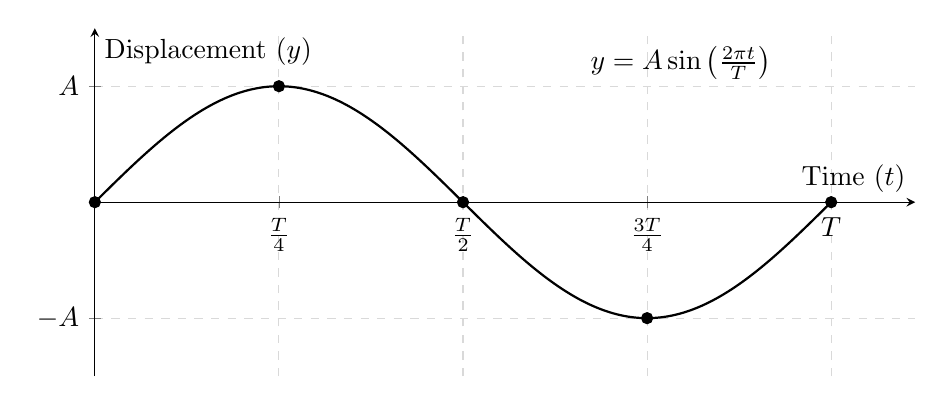
\begin{tikzpicture}
    \begin{axis}[
        width=12cm,
        height=6cm,
        axis lines=center,
        xlabel={Time $(t)$},
        ylabel={Displacement $(y)$},
        xmin=0, xmax=7,
        ymin=-1.5, ymax=1.5,
        xtick={0, 1.5708, 3.14159, 4.7124, 6.2832},
        xticklabels={0, $\frac{T}{4}$, $\frac{T}{2}$, $\frac{3T}{4}$, $T$},
        ytick={-1, 0, 1},
        yticklabels={$-A$, 0, $A$},
        samples=200,
        domain=0:6.2832,
        grid=major,
        grid style={dashed, gray!30},
      ]

      % Plot sine wave
      \addplot[thick, black] {sin(deg(x))};

      % Mark key points
      \addplot[mark=*, mark size=2pt, black] coordinates {(0, 0)};
      \addplot[mark=*, mark size=2pt, black] coordinates {(1.5708, 1)};
      \addplot[mark=*, mark size=2pt, black] coordinates {(3.14159, 0)};
      \addplot[mark=*, mark size=2pt, black] coordinates {(4.7124, -1)};
      \addplot[mark=*, mark size=2pt, black] coordinates {(6.2832, 0)};

      % Function label
      \node at (axis cs:5, 1.2) {$y = A\sin\left(\frac{2\pi t}{T}\right)$};

    \end{axis}
  \end{tikzpicture}

  \caption{Sinusoidal oscillation showing one complete period $T$ with amplitude $A$.}
  \label{fig:sine_oscillation}
\end{figure}

\newpage

\subsection{Formulas}

Now Formulas, a basic \textbf{Quadratic Equation} cheatcode formula

\[
  x = \frac{-b \pm \sqrt{b^{2} - 4ac}}{2a}
\]

\vspace{10pt}

\subsection{Theorems}

\begin{theorem}
  For all $a,b \in \mathbb{R}$, $(a+b)^2 = a^2 + 2ab + b^2$.
\end{theorem}
